
\begin{itemize}
    \item \textbf{HTML}: Separate content and style by using CSS.
    \item \textbf{Browser}: Show information and not the part of the file 
        which say how to show information.

    \item \textbf{Delivering document} 
        \begin{enumerate}
            \item Peer to peer model
            \item Client/server model where a 
                server is a machine that offer services to other machine.

                Note that state must be maintain when request are related. 
                \begin{itemize}
                    \item Client side: It's better to keep state on client side to avoid DoS.
                    \item Server: If state is on the server and multiple server are used,
                    they must be able to exchange state information.
                \end{itemize}

                \paragraph{Concurrency}
                \begin{itemize}
                    \item Thread pools: keep a thread pool with a fixed number of 
                        worker threads
                    \item Event-driven: server's work is driven by events
                        which need a single thread.
                \end{itemize}

                Event-driven servers typically have better performance
                and do not need as much synchronization but
                thread-based are easier to write and maintain.

                \paragraph{Multiple machine}
                Need a proxy to load balance request across machines.

        \end{enumerate}

    \item \textbf{Uniform  Resource  Identifier (URI)} which comme in two form:
        \begin{enumerate}
            \item Uniform  Resource  Name (URNs): \textit{What} to find
            \item Uniform  Resource  Locator (URLs): \textit{Where} to find
        \end{enumerate}

    \item \textbf{DNS}: Hierarchical namespace

        \begin{tabular}{m{5cm}m{11cm}}
            Authoritative  server  knows,  for  each  name  in  its  zone,  which
            machine  corresponds  to  a  given  name,  or  which  other  name  server
            is  responsible.
            &
            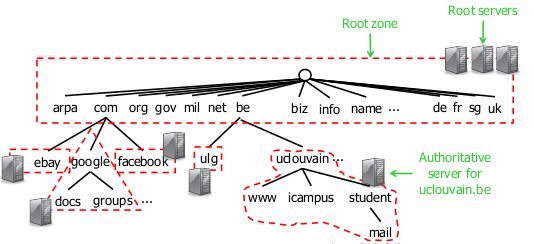
\includegraphics[width=11cm]{img/dns}
        \end{tabular}

    \item \textbf{HTTP}: is a simple stateless protocol
        which use request/response that contain headers used to
        exchange additional information.

        \begin{enumerate}
            \item GET: retreive document
            \item HEAD: Get metadata for a specific document
            \item POST: Add information to a document (as form)
            \item PUT, DELETE
        \end{enumerate}

    \item \textbf{Dynamic content}:

        \paragraph{Document Object Model} (DOM)
        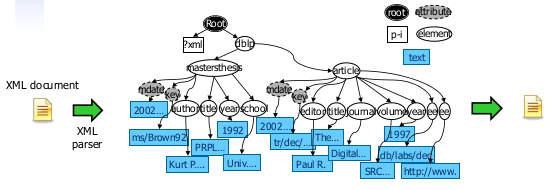
\includegraphics[width=11cm]{img/dom}

        \paragraph{XMLHttpRequest}
        It's a JavaScript  object  that  enables  web  pages  
        to  dynamically and asynchronously  load  more  content. 

        \paragraph{Event handlers}
        Events  can  be  requested  from  the  web  page
        or  directly  from  JavaScript.

        \begin{itemize}
            \item Server-side
                \begin{itemize}
                    \item Web app
                        \begin{enumerate}
                            \item Common Gateway Interface (CGI). When
                                dynamic content is requested:
                                (1) the web server prepare metadata and user-submitted
                                data, (2) runs an external program that produce the web page and
                                (3) return the web page produce by program to the client
                            \item Java servlets: servlets implement a specific
                                method that is given request. They also run one
                                \textbf{servlet container} and each request is its own
                                thread.
                        \end{enumerate}

                        \begin{center}
                            \begin{tabular}{l|cc}
                                & CGI & Servlets \\
                                \hline
                                Request handled by & Processes & Threads \\
                                Copies of code & Potentially many & One \\
                                Session state stored & File System & Servelt container \\
                                Security & Problematic & Handled by Java sandbox \\
                                Portability & Varies & Java \\
                            \end{tabular}
                        \end{center}

                    \item Node.js which is a event-driven programming model, so there
                        is a single thread which must never block. 

                        Note that Express are minimal and flexible framework for writing
                        web app in node.js and EJS allow to write \textit{page templates}.

                \end{itemize}


            \item Client-side
                \begin{itemize}
                    \item JavaScript: Can be embed entirely in HTML or attach in
                        a separate file.

                    \item Ajax: \textit{Asynchronous JS and XML},...
                        \begin{description}
                            \item[+] Much more responsive than plain HTML
                            \item[-] Difficult to integrate navigation element (back button),
                                to accommodate search engine, some compatibility issues
                        \end{description}
                        \begin{center}
                            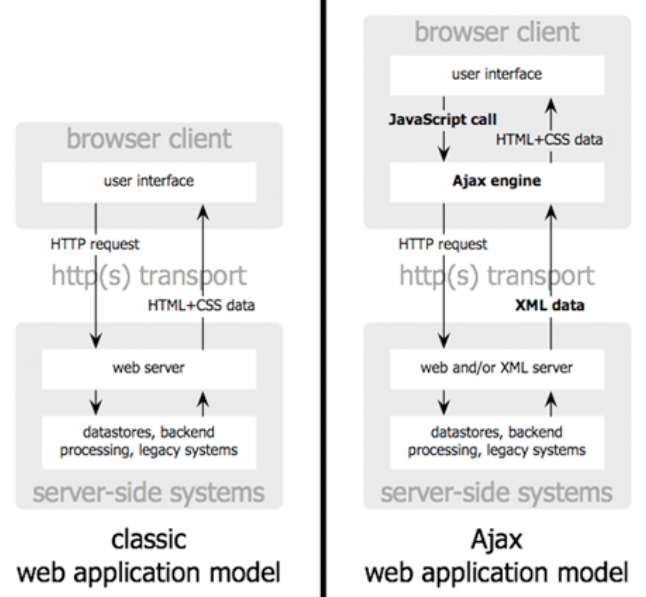
\includegraphics[width=9cm]{img/ajax}
                        \end{center}
                \end{itemize}
        \end{itemize}

    \item \textbf{Session management}
        \begin{itemize}
            \item Use session ID in part of every URL:
                \begin{enumerate}
                    \item URL rewriting by append session ID
                        $$<a  href="foo.html">  \rightarrow <a  href="foo.html?sid=012345">$$
                    \item hidden session ID variables in the HTML
                        $$<input  type="hidden"  name="sid"  value="012345">$$
                \end{enumerate}

            \item Use cookies which is a set of key-­value pairs that a web
                site can store in your browser which is send with \texttt{set-cookie header}
                in HTTP response.

                \paragraph{Note}
                Each cookies as an expiration date, a domain and a
                path. Browser  only  sends  the  cookies  whose  path  
                and  domain  match  the  requested  page.

                \paragraph{Issue}
                Cookie persist and can have some useful information such as
                password.
        \end{itemize}
\end{itemize}


